\documentclass{article}
\usepackage{amsmath,amsthm,amssymb}
\usepackage{mathtext}
\usepackage[T2A]{fontenc}
\usepackage[utf8]{inputenc}
\usepackage[english, russian]{babel}
\usepackage{graphicx}
\usepackage{hyperref}
\usepackage{listings}
\usepackage{color}
\usepackage{float}
\usepackage{bera}% optional: just to have a nice mono-spaced font
\usepackage{xcolor}
\usepackage[nottoc]{tocbibind}

\title{NLP Course 2025. NER по сводкам Министерства Обороны РФ.
}
\author{Андрей Павлов}
\date{May 2025}

\definecolor{maroon}{rgb}{0.5,0,0}
\definecolor{darkgreen}{rgb}{0,0.5,0}
\lstdefinelanguage{XML}
{
  basicstyle=\ttfamily,
  morestring=[s]{"}{"},
  morecomment=[s]{?}{?},
  morecomment=[s]{!--}{--},
  commentstyle=\color{darkgreen},
  moredelim=[s][\color{black}]{>}{<},
  moredelim=[s][\color{red}]{\ }{=},
  stringstyle=\color{blue},
  identifierstyle=\color{maroon}
}

%Define Colors
\definecolor{gray}{HTML}{666666}		%#666666
\definecolor{lightbule}{HTML}{006699}		%#006699
\definecolor{lightgreen}{HTML}{669900}		%#669900
\definecolor{bluegreen}{HTML}{33997e}		%#33997e
\definecolor{magenta}{HTML}{d94a7a}		%#d94a7a
\definecolor{orange}{HTML}{e2661a}		%#e2661a
\definecolor{purple}{HTML}{7d4793}		%#7d4793
\definecolor{green}{HTML}{718a62}		%#718a62

\lstdefinelanguage{json}{
  %keyword1&2&6
  morekeywords = [1]{abstract, class, continue, default, enum, extends, false, final, finally, implements, import, instanceof, interface, native, new, null, package, private, protected, public, static, strictfp, throws, transient, true, void, volatile, length, assert, case, return, super, this, throw},
  %keyword3
  morekeywords = [2]{catch, do, for, if, else, switch, synchronized, while, try},
  %keyword4
  morekeywords = [3]{width, height, pixelHight, displayHeight, displayWidth, focused, frameCount, frameRate, key, keyCode, keyPressed, mouseButton, mousePressed, mouseX, mouseY, pixels, pixelWidth, pmouseX, pmouseY},
  %keyword5
  morekeywords = [4]{Array, ArrayList, Boolean, Byte, BufferedReader, Character, Class, Double, Float, Integer, HashMap, PrintWriter, String, StringBuffer, StringBuilder, Thread, boolean, byte, char, color, double, float, int, long, short, FloatDict, FloatList, IntDict, IntList, JSONArray, JSONObject, PFont, PGraphics, PImage, PShader, PShape, PVector, StringDict, StringList, Table, TableRow, XML},
  keywordstyle = [1]\color{bluegreen},
  keywordstyle = [2]\color{lightgreen},
  keywordstyle = [3]\color{magenta},
  keywordstyle = [4]\color{orange},
  sensitive = true,
  morecomment = [l]{//},
  morecomment = [s]{/*}{*/},
  morecomment = [s]{/**}{*/},
  commentstyle = \color{gray},
  morestring = [b]",
  morestring = [b]',
  stringstyle = \color{purple}
}

\begin{document}
\maketitle
\begin{abstract}
    Ссылка на код проекта: \url{https://github.com/as-pavlov/NLP_2025_RMDR}.
\end{abstract}



\section{Introduction}
В сводках Минообороны РФ о ходе проведения СВО есть статистическая информация о потерях ВСУ, но в свободной форме. Сводки публикуются Минобороны России  на официальном телеграм канале \url{https://t.me/mod_russia}.  Цель проекта с помощью NER (Named Entity Recognition) получить подробные структурированные данные о потерях ВСУ по направлениям и населенным пунктам.
\subsection{Team}

\textbf{Андрей Павлов} подготовил этот документ.



\section{Related Work}
\label{sec:related}
В проекте используются новые данные, и поэтому предыдущих работ по этой теме нет. 



\section{Model Description}
Модель обучалась на базе предобученной модели  Babelscape/wikineural-multilingual-ner взятой с Huggingface. \footnote{ \cite{BSWMN} \url{https://huggingface.co/Babelscape/wikineural-multilingual-ner}}. Файл в котором проводилось обучение модели \verb|NLP_2025_RMDR_NERLM_2.ipynb|. Во время обучения было разморожено 11 последних слоев. В качестве Loss используется CrossEntropyLoss. \cite{NERUB} \cite{HFTC}





\section{Dataset}
Данные для обучения были получены из официального телеграм-канала Министерства обороны РФ \url{https://t.me/mod_russia} путем стандартного экспорта в виде json. В проекте путь к файлу : \verb|ChatExport_2025-04-05\result.json|

В файле \verb|NLP2025_RMDR_GetData.ipynb| проводится предобработка данных, а именно: выделяется "чистый" текст сообщений, удаляются лишние символы. Фильтруются только сообщения о сводках. Подготовленные тексты сохраняются в атрибут clearText объектов message. Результат сохраняется в файл \verb|RMDR.json|

Файл \verb|RMDR.json| размечается в Label Studio с помощью меток.

\subsection*{Описание меток}



\begin{lstlisting}[language=XML]
<View style="display:flex;align-items:start;gap:8px;flex-direction:row">
   <Text name="text" value="$clearText" granularity="word"/>
   <Labels name="label" toName="text" showInline="false">
      <Label value="DIR" background="#4824f9"/>
      <Label value="SLD" background="#00ff1e"/>
      <Label value="WP" background="#ff0000"/>
      <Label value="LOC" background="#57fff4"/>
      <Label value="UNIT" background="green"/>
      <Label value="COUNT" background="#000000"/>
      <Label value="FREE" background="#0008ff"/>
      <Label value="LOST" background="#ff0000"/>
      <Label value="CAPT" background="#ffbb00"/>
  </Labels>
</View>
\end{lstlisting}



\begin{itemize}
  \item DIR - Направление или группа войск
  \item SLD - Солдаты, военнослужащие
  \item WP - Оружие 
  \item LOC - Населенные пункты
  \item UNIT - Штабы, склады оружия и пр.
  \item COUNT - количество (солдат или оружия)
  \item FREE - освобожденные населенные пункты (глаголы)
  \item LOST - утерянные населенные пункты (глаголы)
  \item CAPT - пленные (глаголы)
\end{itemize}

\begin{figure}[H]
    \centering
    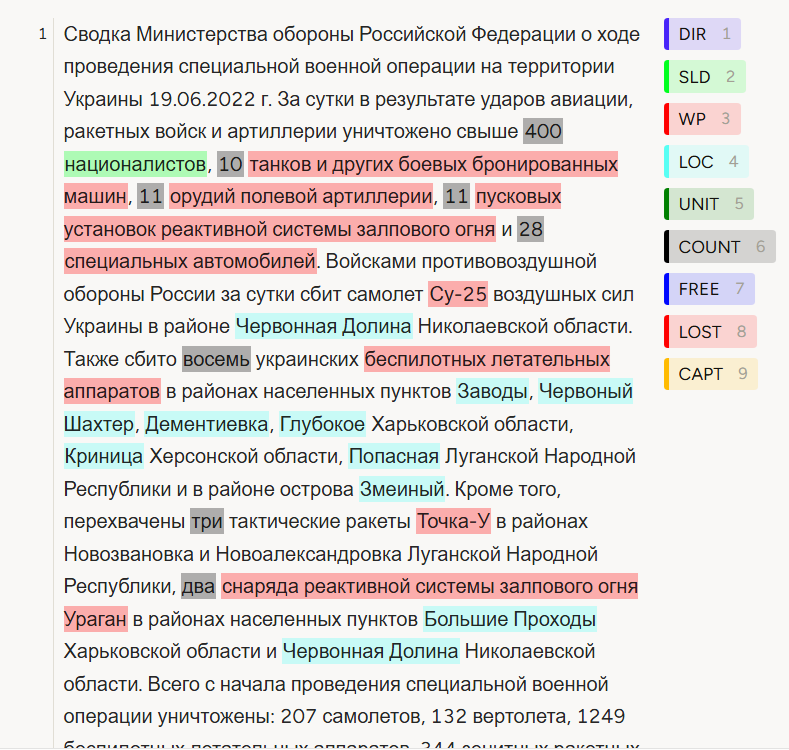
\includegraphics[width=0.9\linewidth]{images/Labal Studio Example.png}
    \caption{Пример разметки в Label Studio}
    \label{fig:enter-label}
\end{figure}

Результаты разметки в Label Studio храняться в файле \verb|RMDR_ANATATION_3_MONTH.json| . 
\footnote{Описание формата анотаций в Label Studio можно посмотреть по этой ссылке \cite{LSJF} \url{https://labelstud.io/blog/understanding-the-label-studio-json-format/}}

В файле размечено только 3 месяца сводок: июнь-июль 2022, июнь 2023, июнь 2024.
При обучении модели ровно эти же данные получаются непосредственно из Label Studio с попощью http запроса GetTasks. Перед обучением данные приводятся к виду:

\begin{lstlisting}[language=json]
        "ids" : torch.tensor(ids, dtype=torch.long),
        "mask" : torch.tensor(mask, dtype=torch.long),
        "token_type_ids" : torch.tensor(token_type_ids, dtype=torch.long),
        "target_tags" : torch.tensor(target_tags, dtype=torch.long)
\end{lstlisting}

\begin{itemize}
  \item ids - Список id токенов, на которые разбит текст
  \item mask - везде 0
  \item \verb|token_type_ids - везде 1| 
  \item \verb|target_tags - id метки для каждого токена. Для токенов для которых нет метки - 0|
\end{itemize}

\section{Experiments}
\subsection{Metrics}
В процессе обучения использовались метрики : precision, recall, accuracy.

\subsection{Experiment Setup}
В процессе обучения данные были разбиты в соотношении 0.9(train) к 0.1 (val).  Так же существенно улучшила результат аугментация данных. Данные разбивались по порциям в 512 токенов (модель больше не может принять), но разбивались со смещением, то есть следующая порция начиналась не с 513 токена, а с 513 -  \verb|SHIFT_SIZE (200)|. 
Так же опытным путем было подобрано количество размороженных слоев, достаточное для хорошего результата.

\subsection{Baselines}
Так как это новые данные (разметка), и использовалась только одна модель, которая показал, хорошие результаты, то других моделей нет и не с чем сравнивать.

\section{Results}
В результате обучения модели удалось добиться следующих значений метрик:

\begin{itemize}
  \item train
    \begin{itemize}
        \item precision = 0.6249239604801263
        \item recall =  0.9428508267145929
        \item accuracy = 0.914273631816007
    \end{itemize}
    \item Val
    \begin{itemize}
        \item precision = 0.6864593295870401
        \item recall =  0.9605542609089559
        \item accuracy = 0.8980305989583334
    \end{itemize}
\end{itemize}

\subsection{Пример результата действия модели}

\textbf{
\subsubsection{Текст}
}

Министерства обороны Российской Федерации о ходе проведения специальной военной операции по состоянию на 5 мая 2025 г.  Вооруженные Силы Российской Федерации продолжают проведение специальной военной операции.  Подразделениями группировки войск Север нанесено поражение скоплениям живой силы и техники механизированной, танковой, егерской бригад ВСУ и двух бригад теробороны в районах населенных пунктов Садки, Рясное, Великая Писаревка Сумской области и Гранов Харьковской области. Потери ВСУ составили до 150 военнослужащих, три танка, две боевые бронированные машины и шесть автомобилей. Уничтожен склад боеприпасов.  Подразделения группировки войск Запад заняли более выгодные рубежи и позиции. Нанесли поражение формированиям двух механизированных, горно-штурмовой, штурмовой бригад ВСУ и бригады теробороны в районах населенных пунктов Пески, Купянск, Григоровка, Кутьковка Харьковской области и Карповка Донецкой Народной Республики. Противник потерял свыше 225 военнослужащих, боевую бронированную машину, шесть автомобилей и два артиллерийских орудия западного производства. Уничтожены три склада боеприпасов.  Подразделения Южной группировки войск улучшили тактическое положение. Нанесли поражение живой силе и технике двух механизированных, аэромобильной бригад ВСУ и бригады теробороны в районах населенных пунктов Серебрянка, Дружковка, Северск и Заря Донецкой Народной Республики. Потери украинских вооруженных формирований составили свыше 315 военнослужащих, две боевые бронированные машины и восемь орудий полевой артиллерии.  Подразделения группировки войск Центр улучшили положение по переднему краю. Нанесли поражение формированиям двух механизированных, егерской бригад ВСУ, бригады спецназначения и двух бригад нацгвардии в районах населенных пунктов Удачное, Димитров, Новопавловка, Новосергеевка и Гродовка Донецкой Народной Республики. Противник потерял до 465 военнослужащих, танк, четыре боевые бронированные машины, шесть автомобилей и четыре артиллерийских орудия.Подразделения группировки войск Восток продолжили продвижение в глубину обороны противника. Нанесли поражение живой силе и технике двух механизированных бригад ВСУ, бригады морской пехоты и бригады теробороны в районах населенных пунктов Богатырь, Федоровка, Комар и Новополь Донецкой Народной Республики. Потери противника составили до 170 военнослужащих, боевая бронированная машина, пять автомобилей и четыре орудия полевой артиллерии. Уничтожены две станции радиоэлектронной борьбы.  Подразделения группировки войск Днепр нанесли поражение формированиям механизированной бригады и двух бригад береговой обороны ВСУ в районах населенных пунктов Малая Токмачка, Павловка Запорожской области и Антоновка Херсонской области. Противник потерял до 70 военнослужащих, пять автомобилей, пусковую установку реактивной системы залпового огня HIMARS производства США и два орудия полевой артиллерии. Уничтожены две станции радиоэлектронной борьбы и склад боеприпасов.  Оперативно-тактической авиацией, ударными беспилотными летательными аппаратами, ракетными войсками и артиллерией группировок войск Вооруженных Сил Российской Федерации поражены объекты инфраструктуры военного аэродрома, ремонтного предприятия авиационной промышленности, склады боеприпасов, а также пункты временной дислокации украинских вооруженных формирований и иностранных наемников в 142 районах.  Средствами противовоздушной обороны уничтожены четыре управляемые авиационные бомбы JDAM и четыре реактивных снаряда системы залпового огня HIMARS производства США, а также 123 беспилотных летательных аппарата самолетного типа.  Всего с начала проведения специальной военной операции уничтожены: 662 самолета,  283 вертолета,  55 452 беспилотных летательных аппарата,  605 зенитных ракетных комплексов,  23 153 танка и других боевых бронированных машин,  1 558 боевых машин реактивных систем залпового огня,  24 435 орудий полевой артиллерии и минометов,  35 005 единиц специальной военной автомобильной техники.

\textbf{
\subsubsection{Результат модели}
}
\begin{itemize}
\item Направление:  Север
    \begin{itemize}
        \item Населенные пункты: Садки, Рясное, Великая Писаревка, Гранов
        \item военнослужащих - 150
        \item танка - три
        \item боевые бронированные машины - две
        \item автомобилей - шесть
        \item склад боеприпасов
    \end{itemize}
\item Направление:  Запад
    \begin{itemize}
            \item Населенные пункты: Пески, Купянск, Григоровка, Кутьковка, Карповка
            \item военнослужащих - 225
            \item боевую бронированную машину
            \item автомобилей - шесть
            \item артиллерийских орудия западного производства - два
            \item склада боеприпасов - три
   \end{itemize}
\item Направление:  Южной
    \begin{itemize}
        \item Населенные пункты: Серебрянка, Дружковка, Северск, Заря
        \item военнослужащих - 315
        \item боевые бронированные машины - две
        \item орудий полевой артиллерии - восемь
   \end{itemize}
\item Направление:  Центр
    \begin{itemize}
        \item Населенные пункты: Удачное, Димитров, Новопавловка, Новосергеевка, Гродовка
        \item военнослужащих - 465
        \item боевые бронированные машины - четыре
        \item автомобилей - шесть
        \item артиллерийских орудия - четыре
   \end{itemize}
  \begin{itemize}
        \item Населенные пункты: Богатырь, Федоровка, Комар, Новополь
        \item военнослужащих - 170
        \item боевая бронированная машина
        \item автомобилей - пять
        \item орудия полевой артиллерии - четыре
        \item станции радиоэлектронной борьбы - две
   \end{itemize}
\item Направление:  Днепр
   \begin{itemize}
      \item Населенные пункты: Малая Токмачка, Павловка, Антоновка
      \item военнослужащих - 70
      \item автомобилей  - пять  
      \item пусковую установку реактивной системы залпового огня HIMARS
      \item орудия полевой артиллерии - два
      \item станции радиоэлектронной борьбы - две
      \item склад боеприпасов,   объекты инфраструктуры военного аэродрома,   склады боеприпасов,   пункты временной дислокации
      районах - 142
      \item управляемые авиационные бомбы JDAM - четыре
      \item реактивных снаряда системы залпового огня HIMARS - четыре
      \item беспилотных летательных аппарата самолетного типа,  - 123
  \end{itemize}
\end{itemize}

Так же в рамках проекта был реализован web service который возвращает результат выполнения модели в формате Label Studio (json). Этот web service можно подключить к Label Studio и использовать его для дальнейшей разметки данных \cite{LSMLB}. Подробнее описано в README.md резозитория.

\section{Conclusion}
В задачи проекта входило получение структурированных данных о потерях ВСУ из сводок Минобороны РФ. Были размечены данные для модели и была обучена модель на этих данных, которая показала хорошие результаты. Также был написан web service, помогающий в дальнейшей разметке данных.

\bibliographystyle{apalike}
\bibliography{lit}
\end{document}
